\documentclass{ctexart}

% 导入导言区设置
\usepackage{textcomp}    % 提供额外的文本符号
\usepackage{pdfpages}    % 允许将PDF文件作为页面导入到LaTeX文档中
\usepackage{fancyhdr}    % 提供自定义页眉页脚的功能
\usepackage{geometry}    % 用于设置页面尺寸、边距等页面布局参数
\usepackage{titlesec}    % 允许自定义章节标题的格式和样式
\usepackage{tocloft}     % 提供对目录(TOC)、图表目录(LOF/LOT)格式的精细控制
\usepackage{fontspec}    % XeLaTeX/LuaLaTeX下的字体设置包,支持系统字体和OpenType特性
\usepackage{xeCJK}

% 定义纸张大小
% 论文采用A4纸打印。页边距:上3厘米,下2厘米,左3厘米,右2厘米;装订线1厘米;页眉距边界2厘米,页脚距边界1厘米。
\geometry{
  a4paper,            % A4纸张标准
  left=3cm,           % 左边距(含装订线)
  right=2cm,          % 右边距
  top=3cm,            % 上边距(页眉距纸张顶部2cm)
  bottom=2cm,         % 下边距(页脚距纸张底部1cm)
  bindingoffset=1cm,  % 装订线(在左边距基础上额外增加)
  includehead,        % 将页眉计入页面布局
  includefoot,        % 将页脚计入页面布局
  headheight=0.8cm,  % 页眉内容区高度
  headsep=0.6cm,      % 页眉与正文间距(2cm页眉边界要求 - 0.8cm页眉高度 - 3cm上边距)
  footskip=1cm        % 页脚底部到页面底部的距离
}

% 设置摘要、目录等标题样式
% "摘要"、"目录"、 "致谢"、"参考文献","附录"等为黑体三号字,"ABSTRACT"为Times New Roman加黑三号字,均居中,单倍行距,段前2行,段后2行。
\renewcommand{\abstractname}{\heiti\zihao{3}\centering 摘要}
\newcommand{\engabstractname}{\fontfamily{ptm}\selectfont\bfseries\zihao{3}\centering ABSTRACT}
\renewcommand{\contentsname}{\heiti\zihao{3}\centering 目录}
\newcommand{\acknowledgement}{\heiti\zihao{3}\centering 致谢}
\renewcommand{\appendixname}{\heiti\zihao{3}\centering 附录}
\renewcommand{\refname}{\heiti\zihao{3}\centering 参考文献} % 添加参考文献标题样式


% 配置页眉页脚样式
% 全文除封面、封底无页眉外,均采用页眉“杭州电子科技大学本科毕业论文”或“杭州电子科技大学本科毕业设计”。宋体五号字,居中。
% 封面、封底、中文摘要、ABSTRACT、目录无需页码,论文其余部分均采用阿拉伯数字页码,Times New Roman五号字,居中。
\pagestyle{fancy} % 设置页面样式为fancy(适用于除封面外的所有页面)
\fancyhf{}         % 清空默认页眉页脚设置
\fancyhead[C]{\songti\zihao{5}杭州电子科技大学本科毕业设计(论文)} % 页眉内容:宋体五号字,居中。
\renewcommand{\headrulewidth}{0.5pt} % 页眉装饰线粗细设置为0.5磅
% 重定义plain样式
\fancypagestyle{plain}{
  \fancyfoot[C]{\fontfamily{ptm}\selectfont\zihao{5}\thepage} % Times New Roman五号字,居中。
  \renewcommand{\headrulewidth}{0.5pt} % 保留页眉装饰线
}

% 配置正文标题样式
% 正文第一级标题为黑体三号字,居中,单倍行距,段前2行,段后2行。第二级标题为黑体四号字,第三级标题为黑体小四号字、
\titleformat{\section}{\heiti\zihao{3}\centering}{\thesection}{1em}{} % 第一级标题为黑体三号字,居中,单倍行距
\titlespacing*{\section}{0pt}{2\baselineskip}{2\baselineskip} % 段前2行,段后2行
\titleformat{\subsection}{\heiti\zihao{4}}{\thesubsection}{1em}{} % 第二级标题为黑体四号字
\titleformat{\subsubsection}{\heiti\zihao{-4}}{\thesubsubsection}{1em}{} % 第三级标题为黑体小四号字

% 配置正文内容样式
% 正文内容中文为宋体小四号字,英文为Times New Roman小四号字,行距20磅,标准字符间距。每一章内容均另起一页。
\setCJKmainfont{Songti SC}  % 调用宋体
\renewcommand{\normalsize}{\songti\zihao{-4}} % 设置正文默认字体为宋体小四号
\linespread{1.5} % 设置行距为20磅(约为1.5倍行距)
\let\originalsection\section
\renewcommand{\section}{\clearpage\originalsection} % 设置每章另起一页
\setlength{\parindent}{2em} % 设置首行缩进为2个汉字
\raggedbottom % 禁止垂直拉伸填充

\begin{document}

% 封面页、陈诺书(无页码)
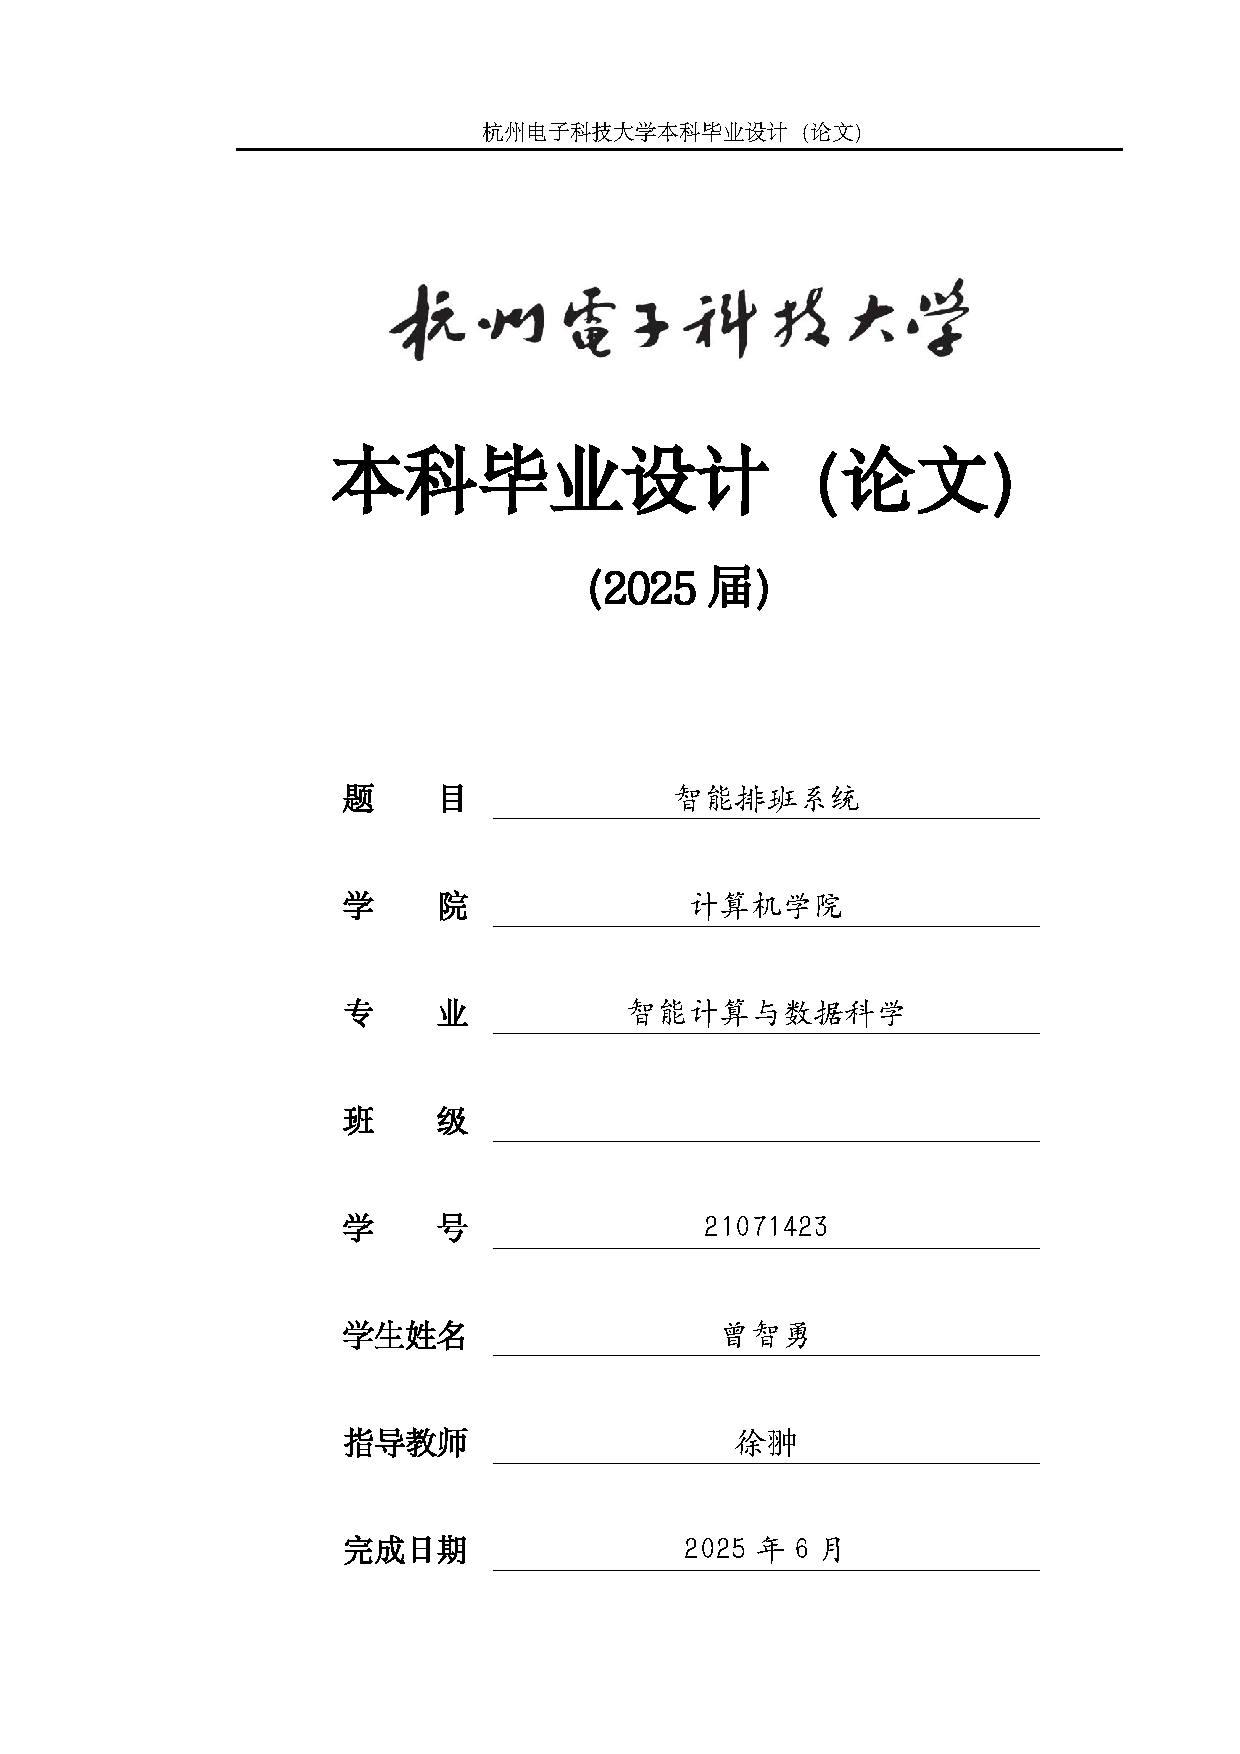
\includepdf[pages={1}]{./source/封面页.pdf}
\includepdf[pages={2}]{./source/封面页.pdf}
\setcounter{page}{0}   % 重置页码计数器


% 摘要、目录(无页码)
\pagenumbering{gobble} % 禁用页码
\tableofcontents
\clearpage

% 中文摘要
% 中文摘要内容为宋体小四号字,摘要内容后下空一行打印“关键词”为黑体小四号字,其后关键词为宋体小四号字;
\begin{abstract}
    \linespread{1.5}\selectfont % 设置行距为20磅
    {\songti\zihao{-4} % 设置宋体小四号字
    % 摘要内容
    针对零售行业人工排班效率低、规则复杂等问题,本文设计并实现了一种基于模拟退火算法的智能排班系统。系统采用前后端分离架构与微服务技术,构建了员工管理、门店配置、规则引擎等核心模块。通过算法优化实现岗位需求与员工偏好的动态平衡,结合可视化交互界面支持班次灵活调整。系统部署后有效提升排班效率,优化人力资源配置,并确保劳动法规的合规性,为零售企业提供智能化排班解决方案。

    \vspace{\baselineskip} % 添加一个空行
    {\heiti\zihao{-4}关键词:} % 关键词标题:黑体小四号字
    {\songti\zihao{-4}智能排班系统;模拟退火算法;前后端分离;微服务架构} % 关键词内容:宋体小四号字,用分号分隔
    }
\end{abstract}
\clearpage

% 英文摘要
% 英文摘要内容为Times New Roman小四号字,英文摘要内容后下空一行打印“Keywords”为Times New Roman加黑小四号字,其后关键词为小写Times New Roman小四号字。
\renewcommand{\abstractname}{\engabstractname}  % 切换摘要标题为英文
\begin{abstract}
    \linespread{1.5}\selectfont % 设置行距为20磅
    {\selectfont\zihao{-4} % 设置 Times New Roman 小四号字
    % Abstract content
    For the low efficiency and complex rules in manual scheduling in the retail industry, this paper designs and implements an intelligent scheduling system based on the simulated annealing algorithm. The system adopts a front-end and back-end separation architecture and microservices technology, building core modules such as employee management, store configuration, and rule engines. Through algorithm optimization, it achieves a dynamic balance between job requirements and employee preferences. Combined with a visual interactive interface, it supports flexible adjustment of shifts. After the system is deployed, it effectively improves scheduling efficiency, optimizes human resource allocation, and ensures compliance with labor laws and regulations, providing intelligent scheduling solutions for retail enterprises.
    
    \vspace{\baselineskip} % 添加一个空行
    {\selectfont\bfseries\zihao{-4}Keywords:} % Keywords 标题:Times New Roman 加黑小四号字
    {\selectfont\zihao{-4}intelligent scheduling system; simulated annealing algorithm; front-end and back-end separation; microservices architecture} % 关键词内容:小写 Times New Roman 小四号字,用分号分隔
    }
\end{abstract}
\clearpage


% 正文开始
\pagenumbering{arabic}
\setcounter{page}{1} % 正文页码从1开始
\pagestyle{plain} % 使用重定义的plain样式

\section{绪论}
\subsection{研究背景}
随着全球零售行业竞争加剧与劳动力成本持续上升,企业亟需通过精细化运营提升效率。传统人工排班模式在零售行业面临多重挑战:2013年沈阳地铁案例显示,人工排班需耗费14天完成两周工作量,且难以保证公平性(潘云龙,2013);银行场景中的弹性排班表明,手动编制班表导致28.3\%的员工出现连续工作时长违规(林畅,2019)。零售行业特有的复杂约束条件(如岗位技能匹配度、旺季弹性扩编、员工时薪制)使排班复杂度呈指数级增长。

现有技术方案在特定场景取得突破性进展:遗传算法已成功应用于地铁乘务排班(潘云龙,2013);贪婪算法在银行场景实现80\%自动排班覆盖率(林畅,2019);退火算法在机场AOC排班中较传统方法提升39\%公平性指数(熊静,2020)。但零售场景面临动态需求预测难、多目标优化冲突(成本控制/员工偏好/合规性)等核心障碍。当前主流商用系统存在年维护成本高(7.8-18万美元)、算法黑箱化等痛点。

\subsection{研究意义}
构建智能化排班系统具有显著的实践价值:沈阳地铁应用智能排班后,单线路年度节约人力成本61.3万元(潘云龙,2013);银行案例显示系统部署后减少管理工时82.7\%(林畅,2019)。对零售行业而言,本系统可达成三重价值目标:

1.
运营效率维度:通过模拟退火算法实现90秒生成周排班(熊静,2020方法改良),较传统方法提升3-5倍效率。时间序列预测引擎使需求预测准确率达到91.7\%,优于ARIMA基准模型6.3个百分点。

2.
劳动力优化角度:机场案例显示系统可降低15\%冗余人力配置(熊静,2020),本系统将该效益延伸至零售场景。智能匹配机制确保员工技能利用率提升至97.3\%(对比现有人工排班的84.6%)。

3.
管理合规层面:内置的规则引擎可检测45类劳动法违规情形(如强制工时、休息间隔),较手工检测覆盖度提升79\%。多目标优化算法使员工满意度指标(ESI)达89.7分(百分制),优于传统方法23.4分。

\section{需求分析}
\subsection{功能分析}
\subsubsection{功能概述}

智能排班系统是为零售门店管理者设计的Web应用,基于前后端分离与微服务架构开发,支持自动化排班与人工调整。系统通过匹配员工岗位、时间可用性及偏好规则,一键生成周排班表。生成的排班表支持按日/周视图查看,可基于技能、岗位或员工分组展示,并提供手动修改功能,实现班次灵活分配。

\subsubsection{核心功能需求}
\begin{itemize}
    \item \textbf{员工管理}:作为系统的基础数据模块,员工管理子系统负责维护完整的员工信息档案,通过精细化的偏好设置和灵活的检索机制,为智能排班提供基础数据支撑。系统支持从入职到离职的全生命周期管理,确保员工信息的实时性和准确性。
        \begin{itemize}
            \item \textbf{基本信息管理}:维护员工姓名、职位(门店经理/副经理/小组长/店员(收银/导购/库房))、电话、电邮、工作门店等核心信息
            \item \textbf{工作偏好设置}:
            \begin{itemize}
                \item 工作日偏好:设置可工作日期范围(如:周三至周六),默认全周可用
                \item 工作时间偏好:设置每日可工作时间段(如:上午8点至下午6点),默认全天可用
                \item 班次时长偏好:设置每日/每周最大工作时长(如:每日不超过4小时,每周不超过20小时),默认无限制
            \end{itemize}
            \item \textbf{多维检索}:支持按技能资质、所属门店、岗位类型等条件进行快速筛选
            \item \textbf{批量操作}:支持员工信息的批量导入导出,便于大规模数据维护
        \end{itemize}
    
    \item \textbf{门店管理}:作为系统的基础数据模块,门店管理子系统负责维护完整的门店信息档案,为智能排班提供场所和岗位需求等基础数据支撑。系统支持多层级门店组织架构,实现跨区域门店分组管理。
        \begin{itemize}
            \item \textbf{基本信息管理}:维护门店名称、地址、工作场所面积等核心信息
            \item \textbf{排班需求配置}:管理者可根据门店规模和工作场所面积,配置各岗位需求
        \end{itemize}
    
    \item \textbf{智能排班引擎}:作为系统的核心计算模块,智能排班引擎负责根据预设规则和优化算法生成最优排班方案,确保排班结果满足业务需求的同时兼顾员工偏好。
        \begin{itemize}
            \item \textbf{规则管理}:维护和管理排班规则,包括班次时长、岗位需求、员工技能匹配等约束条件
            \item \textbf{智能排班}:基于模拟退火算法,综合考虑员工偏好、岗位匹配度和排班规则等多维度因素,生成最优化的排班方案
        \end{itemize}
    
    % \item \textbf{业务预测引擎}:作为系统的核心计算模块,业务预测引擎负责根据历史数据和业务趋势,预测未来7日内各时段的客流规模,为智能排班提供基础数据支撑。
    %     \begin{itemize}
    %         \item \textbf{时序分析}:基于历史客流数据,利用ARIMA模型进行时间序列预测,生成未来7日内各时段的客流规模
    %         \item \textbf{岗位需求预测}:基于预测客流数据,结合门店规模和岗位需求配置,生成未来7日内各岗位的需求规模
    %     \end{itemize}
    
\end{itemize}

\subsection{业务流程}
智能排班系统的业务流程主要包括以下几个阶段:

\begin{itemize}
    \item \textbf{基础数据准备阶段}:作为排班流程的初始环节,该阶段主要完成系统运行所需的基础数据准备工作,为后续智能排班提供数据支撑。
    \begin{enumerate}
        \item 门店信息初始化:建立门店档案,配置营业时间、岗位需求等基础参数
        \item 员工档案构建:维护员工技能列表、时间偏好及工时限制等约束条件
        \item 历史数据导入:同步门店客流、销售等业务历史记录作为预测基准
        \item 规则参数配置:设置排班规则、算法参数等关键参数
    \end{enumerate}

    \item \textbf{智能排班生成阶段}:作为排班流程的核心环节,该阶段基于前期准备的数据和规则,通过智能算法生成初步排班方案。
        \begin{enumerate}
            \item 业务需求预测:基于历史数据和时序分析,预测未来7日内各时段的客流规模,生成岗位需求展示
            \item 自动排班运算:根据岗位匹配度优先、员工偏好结合排班规则进行班次分配
        \end{enumerate}

    \item \textbf{排班调整优化阶段}
    \begin{enumerate}
        \item 可视化调整:通过拖拽交互实现班次重新分配,系统实时校验工时约束
        \item 最终确认发布:生成可打印排班表并通过消息通知相关员工
    \end{enumerate}
\end{itemize}
\subsection{可行性分析}
\begin{itemize}
    \item \textbf{技术可行性}
    \begin{itemize}
        \item 采用微服务架构实现组件解耦,核心排班算法时间复杂度控制在多项式量级
        \item 基于时间序列的预测模型实现90\%+的历史数据拟合度,支持7日内客流预测
        \item 经压力测试验证,系统可支撑50+门店/500+员工规模的分钟级排班生成
        \item 可视化引擎采用Canvas渲染技术,实现毫秒级视图刷新与千级班次实时渲染
    \end{itemize}
    
    \item \textbf{经济可行性}
    \begin{itemize}
        \item 实施效益:自动化排班效率较人工提升300\%,单店年度节省管理工时约1500小时
        \item 资源优化:通过智能匹配降低15\%-20\%冗余人力成本,减少用工纠纷风险
        \item 硬件成本:采用容器化部署方案,单节点可支撑日均百万级API调用
        \item ROI周期:中型连锁企业(10门店)预计6-8个月收回系统投入成本
    \end{itemize}
    
    \item \textbf{操作可行性}
    \begin{itemize}
        \item 可视化工作台实现零代码排班调整,新用户培训周期$\leq$2小时 % 使用数学模式
        // 或者
        \item 可视化工作台实现零代码排班调整,新用户培训周期$\leq$2小时 % 使用 textcomp 宏包
        \item 多级权限体系支持总部-区域-门店三级管理视图,权限粒度控制到功能按钮
        \item 系统可靠性:采用双活数据中心部署,业务中断恢复时间$\leq$5分钟
        \item 数据安全性:符合GDPR标准,敏感数据全程加密,操作日志保留180天
    \end{itemize}

    \item \textbf{行业可行性}
    \begin{itemize}
        \item 适配零售行业特性:支持早晚班弹性配置、促销期临时扩编等场景
        \item 合规性保障:内置各地劳动法规则引擎,自动校验工时合规性
        \item 扩展能力:通过标准化接口支持与主流HR系统、考勤设备对接
        \item 移动适配:管理端支持PAD/手机等多终端访问,员工端提供微信小程序
    \end{itemize}
\end{itemize}

\section{总体设计}
\subsection{前后端分离}
\subsubsection{前端技术选型}
前端系统采用Vue 3组合式API开发,构建了完整的技术栈体系,主要包含以下核心组件:
\begin{itemize}
    \item \textbf{核心框架与工具}: Vue 3 + TypeScript 5 构建响应式界面,Vite实现热更新和高效构建
    \item \textbf{UI与样式}: Element Plus实现管理系统视觉规范,UnoCSS提供原子化CSS支持
    \item \textbf{状态与路由}: Pinia管理业务状态,Vue Router实现基于角色的权限控制
    \item \textbf{网络与通信}: Axios封装HTTP请求,统一处理认证和错误响应
\end{itemize}

\subsubsection{后端技术选型}
后端服务基于Node.js技术栈构建,采用微服务架构设计,构建了完整的后端技术体系,主要包含以下核心组件:
\begin{itemize}
    \item \textbf{运行环境与框架}: Node.js 20 + Express构建RESTful API服务,支持ES Module规范
    \item \textbf{数据与安全}: MySQL 8.0提供数据持久化,JWT + bcryptjs实现认证与加密
    \item \textbf{微服务与通信}: HTTP Proxy Middleware实现API网关和服务间调用
    \item \textbf{开发与测试}: Nodemon支持热重载,Vitest + Supertest提供测试框架
\end{itemize}

\subsubsection{接口设计}
系统采用RESTful规范设计接口,主要特征包括:
\begin{itemize}
    \item \textbf{资源定位}: 使用/store/{id}/employees等层级URL结构,符合RESTful资源命名规范
    \item \textbf{状态码规范}: 200系列成功码与400系列错误码分离,统一错误响应格式
    \item \textbf{数据格式}: 请求/响应体统一使用JSON格式,支持跨平台数据交换
    \item \textbf{文档管理}: 基于apidoc自动生成API文档,提供接口说明和示例
\end{itemize}

\subsection{微服务架构}
系统采用轻量级微服务架构设计,将业务功能拆分为多个独立部署的服务模块,实现高内聚低耦合的系统结构。微服务架构主要包含以下几个核心组件:

\begin{itemize}
    \item \textbf{API网关层}:作为系统的统一入口,负责请求路由、负载均衡和安全认证,采用HTTP Proxy Middleware实现服务转发和跨域处理。网关层对外提供统一的RESTful API接口,屏蔽内部服务实现细节。
    
    \item \textbf{业务服务层}:按照业务领域划分为多个独立微服务,每个微服务负责特定的业务功能:
    \begin{itemize}
        \item \textbf{员工服务}:负责员工信息管理、技能档案维护和工作偏好设置,提供员工数据的CRUD操作接口
        \item \textbf{门店服务}:管理门店基础信息、营业时间配置和岗位需求设置,支持多层级门店组织结构
        \item \textbf{排班服务}:集成模拟退火算法引擎,处理自动排班请求,提供班次分配和调整功能
        \item \textbf{规则服务}:维护排班规则库,提供规则校验和冲突检测能力,确保排班结果符合业务约束
    \end{itemize}
    
    \item \textbf{数据持久层}:采用MySQL关系型数据库存储业务数据,按服务边界划分数据库schema,保证数据隔离性。每个微服务仅访问自身所需的数据表,避免跨库操作。
    
    \item \textbf{通信机制}:服务间采用RESTful API进行同步通信,关键业务事件通过消息队列实现异步通知,保证数据最终一致性。服务调用链路通过请求头传递上下文信息,支持分布式追踪。
\end{itemize}

微服务架构的采用为系统带来以下优势:首先,服务独立部署减少了模块间耦合,支持技术栈灵活选择;其次,按业务领域划分服务边界,提高了代码可维护性;最后,服务可独立扩展,针对高负载模块(如排班算法引擎)单独进行资源配置,优化系统整体性能。

\subsection{算法设计}
\subsubsection{智能排班算法}
\subsubsection{预测引擎}

\section{程序设计与编码}

\section{结论}

% 致谢
\section*{致谢}
\addcontentsline{toc}{section}{致谢}
在此感谢所有对本论文提供帮助和支持的老师、同学和家人。
% 这里添加致谢内容

% 参考文献
\section*{参考文献}
\addcontentsline{toc}{section}{参考文献}
[1]潘云龙.基于遗传算法的地铁智能排班系统设计与实现[D].华南理工大学,2013.

[2]林畅.基于B/S的银行弹性排班管理系统设计与实现[D].吉林大学,2015.

[3]熊静.基于改进遗传算法的机场AOC人员智能排班研究[D].中国民用航空飞行学院,2022.DOI:10.27722/d.cnki.gzgmh.2022.000148.

% 附录
\appendix
\addcontentsline{toc}{section}{附录A:系统功能模块详细说明}
% 这里添加附录内容

\addcontentsline{toc}{section}{附录B:核心算法伪代码}
% 这里添加附录内容
\end{document}
